\chapter{Physical Modeling}

\section{Processi Fisici Generatori di Suono}
Si modellano tutti i processi fisici che portano alla generazione sonora:

\subsection{Circuiti Elettronici Analogici}
\begin{itemize}
  \item Oscillatori
  \item Sorgenti caotiche
  \item Filtri
  \item Circuiti optoelettrici
\end{itemize}

\subsection{Sistemi Acustici}
\begin{itemize}
  \item Tubi (1D)
  \item Corde (1D)
  \item Piastre (2D)
  \item Stanze (3D)
\end{itemize}

\section{Tipi di Processi Fisici}
I processi fisici di interesse sono lineari, non lineari o addirittura caotici:

\begin{itemize}
  \item Propagazione delle onde (solitamente isotrope e lineari) e generazione di onde stazionarie in un mezzo o in un risonatore
  \item Eccitazione di un risonatore
  \item Interazione rigida/elastica non lineare tra corpi
\end{itemize}

\section{Modellazione a Tempo Continuo e Discreto}
\begin{itemize}
  \item Generalmente un modello a tempo continuo è derivato in termini di equazioni differenziali
  \item Questi possono essere estremamente complessi per essere risolti in tempo reale, si possono applicare delle approssimazioni
  \item Un esempio di approssimazione è la teoria modale
  \item Viene quindi derivato un modello a tempo discreto per eseguire il calcolo su un computer
\end{itemize}

\section{Domini Fisici e Variabili}
Tutti i domini fisici di interesse sono descritti da quantità misurabili che di solito si presentano in coppie di variabili:

\begin{itemize}
  \item Meccanica: Forza + Velocità
  \item Acustica: Pressione + Velocità del volume
  \item Elettrico: Tensione + Corrente
  \item In generale: variabile "trasversale" (o "potenziale") + variabile "passante" (o "cinetica")
\end{itemize}

La tensione è il potenziale "attraverso" due terminali e la corrente è il flusso di elettroni "attraverso" una sezione.

\section{Paradigmi di Modellazione}
\subsection{Paradigma 1: K-variables}
K-variables, o Kirchhoff variables: utilizza la coppia «across» e «through» (trasversale e passante)

\begin{itemize}
  \item Questo fornisce una soluzione diretta del sistema
  \item Può essere utilizzato per scomporre il sistema nei suoi modi naturali
\end{itemize}

\subsection{Paradigma 2: W-variables}
Astrazione: utilizzare il concetto astratto di "onde".

\begin{itemize}
  \item Variabili W, o variabili d'onda: onde incidenti e riflesse
  \item Le onde sono astrazioni che si sommano per comporre le grandezze osservabili K
\end{itemize}
\section{1D Wave Eq. and Solutions}

\subsection{Digital Waveguides}

\begin{itemize}
  \item I Digital Waveguides seguono l’approccio W-domain, ma non devono essere confusi con gli Wave-Digital Filters.
  \item Forniscono un modo molto economico per modellare la propagazione delle onde in condizioni ideali per problemi 1D.
  \item Per problemi 2D e 3D possono essere impiegati, ma il costo computazionale non è più conveniente rispetto ad altri approcci.
\end{itemize}

\section{Caso 1D}

La propagazione di una grandezza \( y \) in un mezzo, ad esempio la propagazione di un'onda di velocità in una corda rigida ideale, può essere modellata come:

\[
\frac{d^2 y}{dt^2} = c^2 \frac{d^2 y}{dx^2}
\]

dove \( c \) è la velocità di propagazione.

\subsection{Soluzione a questa PDE}

La prima soluzione a questa equazione alle derivate parziali (PDE) fu data da D'Alembert nel 1747:

\[
y(x, t) = y^+ \left( t - \frac{x}{c} \right) + y^- \left( t + \frac{x}{c} \right)
\]

Ciò significa che il valore della variabile al tempo \( t \) e nella posizione \( x \) può essere calcolato dalla sovrapposizione di due onde viaggianti: un'onda progressiva \( y^+ \) e un'onda regressiva \( y^- \) di forma arbitraria.

\section{Somma di Onde Progressive e Regressive}

La soluzione al caso 1D è rappresentata dalla somma di onde progressive e regressive.

\section{Discretizzazione della Soluzione di D'Alembert}

La formulazione dei Digital Waveguides (DWG) è ottenuta mediante discretizzazione della soluzione di D'Alembert. La stringa è discretizzata a intervalli spaziali regolari:

\[
x_m = m \Delta x, \quad m \in \{0, \dots, M\}
\]

Il valore di ogni punto viene calcolato a intervalli di tempo regolari:

\[
t_n = n \Delta t, \quad n \in \{0, \dots, N\}
\]

L'equazione d'onda può quindi essere riscritta come:
\begin{figure}[H]
    \centering
    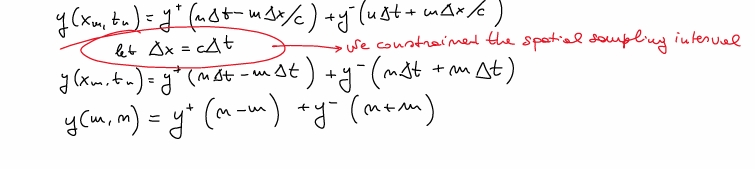
\includegraphics[width=0.7\textwidth]{capitoli/capitolo14/immagini/image1.jpeg}
\end{figure}

\[
\text{(equazione d'onda discretizzata)}
\]

\section{Condizione di Stabilità e Alias Spaziale}

La selezione dell'intervallo di campionamento spaziale è fondamentale per la stabilità e per evitare l'aliasing spaziale. La condizione di stabilità di Von Neumann impone che:

\[
\frac{c \Delta t}{\Delta x} \leq 1
\]

\section{Formulazione DWG e Diagramma di Flusso}

La formulazione dei Digital Waveguides corrisponde al seguente diagramma di flusso:
\begin{figure}[H]
    \centering
    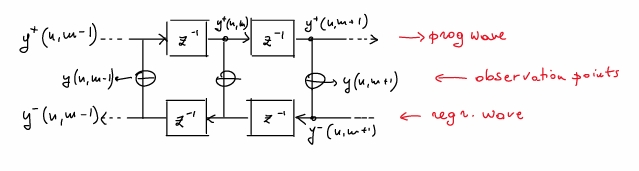
\includegraphics[width=0.7\textwidth]{capitoli/capitolo14/immagini/image2.jpeg}
\end{figure}

\section{Terminazioni "Rigide"}

Le condizioni al contorno sono fondamentali per definire il problema. Un caso tipico è la terminazione rigida: ad esempio, la corda non può muoversi ai suoi estremi. Questo è imposto dall'avere:

\begin{itemize}
  \item Le condizioni di terminazione rigida specificano che la velocità della corda alle estremità sia zero.
\end{itemize}

\section{Aggregazione}

Se possiamo accettare di non calcolare l'uscita in tutte le posizioni, possiamo semplificare il modello utilizzando un approccio di aggregazione:

\begin{itemize}
  \item Si riduce la complessità computazionale, trascurando alcune informazioni spaziali in favore di un'efficienza maggiore.
\end{itemize}

\begin{figure}[H]
    \centering
    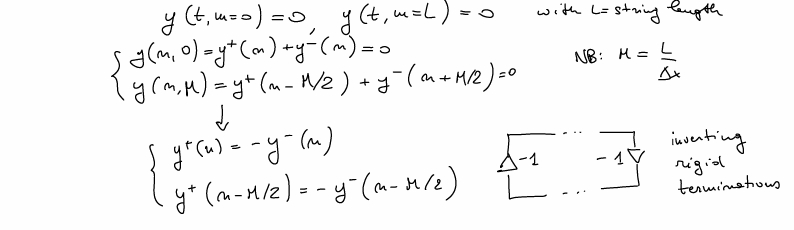
\includegraphics[width=0.7\textwidth]{capitoli/capitolo14/immagini/image3.jpeg}
\end{figure}

\section{Perdite}

In realtà, il mezzo non è privo di perdite e può presentare attriti. La soluzione è ora espressa come onde viaggianti a decadimento esponenziale:

\begin{itemize}
  \item La perdita di energia è modellata come un termine che rappresenta il decadimento esponenziale dell'onda mentre si propaga.
\end{itemize}

\begin{figure}[H]
    \centering
    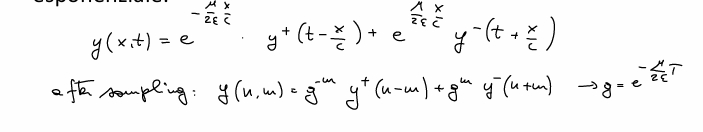
\includegraphics[width=0.7\textwidth]{capitoli/capitolo14/immagini/image4.jpeg}
\end{figure}

\section{Perdite Dipendenti dalla Frequenza}

Il termine di attrito è solo un'approssimazione. È possibile introdurre termini di perdita aggiuntivi per approssimare un comportamento dipendente dalla frequenza. La soluzione si generalizza ora a:

\begin{itemize}
  \item Le perdite dipendenti dalla frequenza sono modellate come un filtro che modula l'attenuazione in funzione della frequenza.
\end{itemize}

\section{Aggregazione di Perdite Dipendenti dalla Frequenza}

I termini dipendenti dalla frequenza possono essere consolidati come un filtro. Questo approccio consente di modellare in modo più preciso le perdite, specialmente in sistemi con comportamento non lineare o con forti variazioni di impedenza.

\begin{itemize}
  \item Utilizzare un filtro permette di simulare in modo efficiente i cambiamenti nelle perdite a seconda della frequenza, migliorando la realismo del modello.
\end{itemize}


\section{Dispersione}

La rigidità di una corda vibrante introduce una forza di ripristino proporzionale alla quarta derivata dello spostamento della corda.

\section{Effetto di Dispersione}

L'effetto di primo ordine della rigidità è l'aumento della velocità di propagazione delle onde con la frequenza:

\[
\omega = \omega_0 \left( 1 + \frac{2K}{c_0^2} \right)
\]

Pertanto, le onde che viaggiano si "disperdono" mentre attraversano la corda. Le componenti ad alta frequenza si propagano più velocemente.

\section{Decomposizione Modale}

L'effetto di dispersione può essere studiato utilizzando una decomposizione modale.

\section{Ritardi Dipendenti dalla Frequenza}

La dispersione richiede ritardi dipendenti dalla frequenza. Se possiamo aggregare, un'opzione conveniente è l'utilizzo di filtri Allpass.

\section{Fractional Delays}

Come intonare una Digital Waveguide (DWG)?

\begin{itemize}
    \item Finché il numero di tappi \( N \in \mathbb{N} \), il numero delle frequenze ottenibili è un insieme discreto.
    \item Per dividere un delay unitario, dobbiamo ricorrere a dei delay frazionari.
\end{itemize}

\section{Discrete-Time Arbitrary Delay}

\begin{figure}[H]
    \centering
    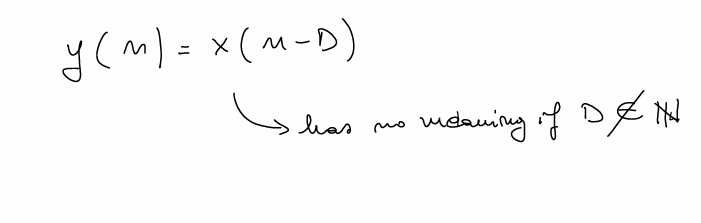
\includegraphics[width=0.7\textwidth]{capitoli/capitolo14/immagini/image5.jpeg}
\end{figure}

L'interpolazione del valore tra due intervalli di campionamento successivi è equivalente alla ricostruzione del segnale a tempo continuo dai valori discreti secondo il campionamento Shannon-Nyquist. Pertanto, l'interpolatore ideale è esattamente il filtro di ricostruzione!

\[
\text{Il fractional-delay ideale è quindi un filtro di ricostruzione.}
\]

%dove mi sono fermato
\section{Discrete-Time Arbitrary Delay}

Quando \( 0 < d < 1 \), l'IR risultante è infinito, non causale e non stabile BIBO (non assolutamente sommabile). Possiamo solo approssimare il ritardo frazionario ideale.

\subsection{Dominio della Frequenza}
Guardando al dominio della frequenza:

\begin{itemize}
    \item Tuttavia, nessun filtro con coefficienti reali può essere complesso a Nyquist.
    \item Questo significa che l'errore di approssimazione sarà almeno \( \sin\left( \frac{\pi D}{2} \right) \), il che è noto come il vincolo di Tarczynski.
\end{itemize}

\section{Fractional Delay Ideale (Tempo Continuo)}

Il ritardo continuo (frazionario) nel tempo e nella frequenza è rappresentato come un filtro ideale di fase lineare all-pass.

\begin{figure}[H]
    \centering
    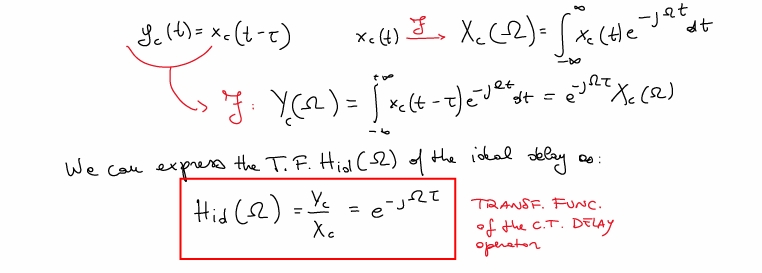
\includegraphics[width=0.7\textwidth]{capitoli/capitolo14/immagini/image6.jpeg}
\end{figure}


\subsection{Caratteristiche in Frequenza}

Il fractional delay ideale è un filtro all-pass di fase lineare.

\begin{figure}[H]
    \centering
    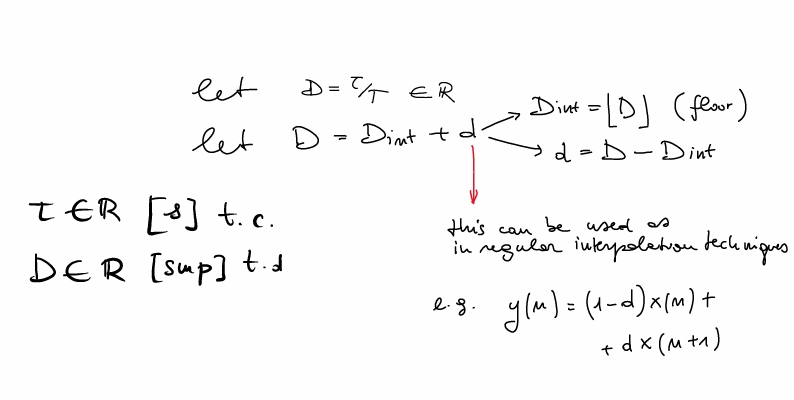
\includegraphics[width=0.7\textwidth]{capitoli/capitolo14/immagini/image7.jpeg}
\end{figure}


\section{Progettazione del Filtro Interpolatore}

Il ritardo frazionario può essere approssimato da un filtro FIR o da un filtro IIR.

\subsection{Metodi di Progettazione FIR}

\begin{itemize}
    \item Troncamento dell'IR, progettazione ai minimi quadrati, approssimazione polinomiale, ecc.
    \item Vantaggi: i coefficienti possono essere modificati senza problemi di stabilità.
\end{itemize}

\subsection{Metodi di Progettazione IIR}

\begin{itemize}
    \item Basato su design all-pass.
    \item Vantaggi: ritardi più elevati con costi di calcolo inferiori.
    \item FLIPPED CLASSROOM: Thiran Allpass.
\end{itemize}

\section{Strumenti ad Ancia}

\begin{itemize}
    \item Se il bore è cilindrico, come nel caso del clarinetto, può essere modellato semplicemente utilizzando una linea di ritardo bidirezionale.
    \item Se il bore è conico, come nel caso del sassofono, può essere modellato come una linea di ritardo bidirezionale, ma l'interfacciamento con esso è più complesso, soprattutto in corrispondenza dell'imboccatura.
    \item Il filtro d'uscita è un filtro peak che definisce la campana di risonanza.
    \item Il filtro di riflessione modella il comportamento in frequenza del bore.
    \item Il modello dell'ancia è essenzialmente una non linearità molto "orizzontale".
\end{itemize}

\section{Strumenti ad Arco}

\begin{itemize}
    \item La coppia di linee di ritardo di destra trasporta i campioni delle onde di velocità di sinistra e di destra (Bridge to Bow delay).
    \item La velocità della corda in qualsiasi punto si ottiene sommando un campione di velocità in direzione sinistra al campione di velocità in direzione destra immediatamente opposto nell'altra linea di ritardo.
    \item Il filtro di riflessione a destra implementa le perdite al ponte, all'archetto, al capotasto o alle terminazioni delle dita (quando sono ferme), e l'attenuazione/dispersione di andata e ritorno dalla corda.
    \item Con un ottimo grado di approssimazione, il nut riflette le onde di velocità in entrata (con un'inversione di segno) a tutte le lunghezze d'onda.
    \item L'interpolazione delle linee di ritardo può essere utilizzata per fornire un cambiamento continuo della posizione dell'arco.
\end{itemize}

\section{Strumenti ad Aria (Flue)}

\begin{itemize}
    \item La generazione sonora è composta dal rumore del "soffio" che entra nella sezione risonante.
    \item La generazione armonica è "arricchita" dalla non linearità \( x - x^3 \) che modella la parte di energia che ritorna dalla canna al momento dell’insorgere della pressione.
    \item Il decadimento in frequenza è dato dal filtro LP nell'anello della "flue bore DL".
    \item La combinazione dell'effetto dei due anelli intona la nota. Tipicamente la DL bore corrisponde alla lunghezza d'onda della nota, mentre la DL dell'imboccatura è metà della DL di bore.
    \item Il modello può essere reso più stabile.
\end{itemize}
